\newpage
\section{Introduction}
\todo[inline]{/{This section shall introduce the reader to the subject addressed by the report. It should include i) a brief explanation of how a brake-by-wire system works and its main advantages and drawbacks compared to existing brake systems, and ii) a description of the purpose of the report, i.e., a formulation of the problem to which the report provides an answer. The last paragraph should consist of a “roadmap” of the report.}/}

The purpose of this laboratory assignment is to gain understanding about how dependability modeling can be applied to evaluate fault-tolerant systems. In this report, two different design solutions for a brake-by-wire systems is evaluated.
 
In a brake-by-wire system, the conventional hydraulic is replaced by an electronic system. The advantage to use a electronic system instead of the conventional is lower weight, lower cost, and simpler integration with other electronic systems already in use, such as active safety systems and stability control. 

The model used for a brake-by-wire system is shown in Fig. \ref{bbwsys}. The central unit (CU) receives the measured brake force intended by the driver and transmits brake command 

%Brake-by-wire systems are expected to replace hydraulic brake systems in future road vehicles. In a brake-by-wire system, the driver’s brake intention is transmitted electronically from the brake pedal to electro-hydraulic or electro-mechanical brake actuators positioned at each wheel. Potential advantages of brake-by-wire systems compared to traditional hydraulic systems include lower cost, lower weight and simpler integration with stability control and active safety systems. 

%Figure 1 shows an overview of the brake-by-wire system. The brake pedal is connected to a central unit (CU). When the driver presses th e brake pedal, the central unit sends messages containing brake commands to each of the four wheel units (WU). To ensure the safety of the system, the central unit and the wheel units must be fault-tolerant. Both the central unit and the wheel units are therefore implemented using redundant computer modules (see Figure 3 and 4). Two serial buses (SB1 and SB2) are provided to ensure fault-tolerance for the data communication. 

%To optimize brake performance, the system executes a closed loop anti-lock braking control algorithm for each wheel. The inputs to the anti-lock control program consist of the current wheel speed and brake force commands generated by a stability control program, which is executed in the central unit. The wheel speed is measured by a wheel speed sensor included in each wheel unit. The input to the stability control program consists of data from several sensors. These sensors measures the position of th e brake-pedal (the driver’s brake intention), the angle of the steering wheel (the driver’s intended direction), the yaw rate (the rotation rate of the vehicle around its y-axis), the roll rate , and the vehicle’s lateral and longitudinal acceleration. In this laboratory class, we will focus our attention on where to execute the anti- lock-braking algorithms. We will not consider the reliability of the sensors used by stability control program.  

%We will investigate two possible implementations of the system. In the first approach, the anti-lock control algorithms are executed locally in the wheel units. The complexity of the wheel units is in this design approximately the same as that of the central unit. However, the failure rate of the wheel units is higher than for the central unit, as they are more exposed to vibrations, moisture and temperature cycling. We call this design approach the distributed architecture. 

%The second approach is to execute the control algorithm for each wheel in the central unit, and let the wheel units consist of simple interfaces to the actuators and sensors. In this case, the control loops for anti-lock braking are closed over the communication network. The advantage with this approach is that the wheel units contain less hardware since they essentially consist of a communication interface, which sends data from the wheel speed sensor and receives commands to the brake actuator. Thus, the failure rate of the wheel units is lower compared to the other design. On the other hand, the failure rate of the central unit is higher, since it requires more processing power and more memory. We call this design approach the centralized architecture , since all control law calculations are performed by the central unit. 

\begin{figure}[h!]
  \centering
  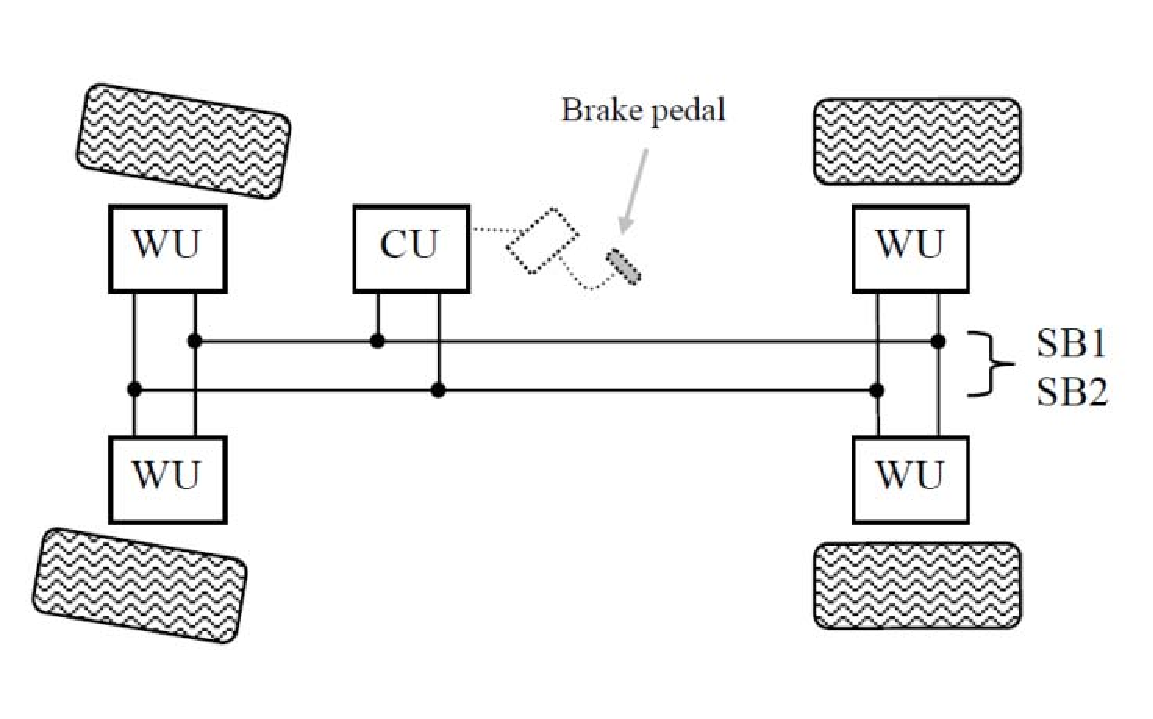
\includegraphics[scale=.5]{Fig1.pdf}
  \caption{Brake-by-wire system}
  \label{bbwsys}
\end{figure}